%%
%
% TODO:
% - talk somewhere about the types of attack which we allow
% - make sure I talk about the types of channel which we use
% Q: where should I talk about Alice's function F?
% - understand the mapping from complex values to binary
% - some more remarks about the running of the protocol?
% - mention somewhere my linestyle convention for different types of channel

\chapter{Quantum secret sharing}
Goal of chapter: introduce our QSS protocol and prove its security in different contexts.

\iffalse
Key results which I want to present:
\begin{itemize}
\item our QSS protocol
\item security proof (what does it do? what does it not do?)
\item analysis of security in various settings - heterodyne, $\mathcal{A}_4$, BS0, BS1, BS2, EC, varying $\alpha$, $T$, $\xi$, $g$, $h$ of both channels
\item show how the protocol performs
\end{itemize}
\fi

\MT{Short introduction to chapter.}

\section{Our QSS protocol}

Our quantum secret-sharing scheme allows for a dealer, Alice, to distribute a classical secret between two recipients, Bob and Charlie. Bob and Charlie should be able to exactly reconstruct the secret when they behave honestly, while a dishonest and unauthorised conspiracy of players--including those outside the protocol--should gain no information. Crucially, although the scheme should allow for dishonesty among the recipients a dishonest player should be forced to collaborate with an honest one.

\begin{figure}[htp]
\centering
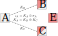
\includegraphics[draft=false, width=0.5\linewidth]{qss/qss_setup_cartoon}
\caption{\label{fig:qss_structure} All quantum secret sharing schemes follow the same structure. Alice encrypts her classical secret $\sigma_A$ with key $K_A$, and broadcasts the resulting $\varsigma_A$. Shares of $K_A$ are distributed among recipients Bob and Charlie such that $K_B \oplus K_C = K_A$. Gray boxes denote honest players, while red denotes dishonest players. The half-red/half-gray boxes denote uncertainty about which player is dishonest. %say somewhere it's all classical?
}
\end{figure}

\subsection{QSS setup}

All QSS protocols follow essentially the same structure, Fig.~\ref{fig:qss_structure}:
\begin{enumerate}
\item Alice (A) uses quantum resources to distribute shares of classical key $K_A$ among recipients Bob (B) and Charlie (C), such that $K_A = K_B \oplus K_C$.
\item Alice encrypts her secret $\varsigma_A = K_A \oplus \sigma_A$ and makes the encrypted secret $\varsigma_A$ publicly known.
\end{enumerate}
The $\oplus$ operation corresponds to bitwise addition (XOR) of binary keys and, provided that $K_A, K_B, K_C$ and $\sigma_A$ are the same length, the above secret sharing operation is provably unconditionally secure \cite{Schneier1996}, provided that key shares $K_B, K_C$ are securely distributed.

This form is similar to QKD-based encryption and it is for this reason that renowned cryptographer Gustavus Simmons wrote that 

\begin{center}\emph{``Secret sharing is simply a special form of key distribution''}\end{center}

\noindent as the abstract to Ref.~\cite{Simmons1990a}.

QSS protocols then only differ in the method used to generate and share the $K_B, K_C$ forming the encryption key. One attractive option would be for Alice to perform individual QKD protocols, first with Bob and then with Charlie, and then XOR the resulting keys together. Since QKD is provably secure, neither Bob nor Charlie can gain sufficient information about the other player's key. The resulting QSS scheme is thus also secure. We discuss this form of QSS at length in Sec.~\ref{sec:intro_qss_lit_review} and again in Chapter~\cite{chapter:aqc}.

Other options for generation and distribution of $K_B, K_C$ are discussed in Sec.~\ref{sec:intro_qss_lit_review} and fall into one of two categories. The first category \cite{Hillery1999, Karlsson1999, Gottesman1999, Markham2008, Wu2016, Kogias2017} relies on large entangled states shared between all $N$ players, while the second category \cite{Zhang2005a, Schmid2005, Schmid2007, Grice2019}, involves distribution of a single (typically one-mode) quantum state between all $N$ players, who each perform their choice of measurement on the state. In both forms, if $N-1$ players communicate and share their choice of measurement and their measurement outcomes, they have sufficient information to infer the measurement outcome of the $N^{\text{th}}$ player. In this way, a key $K_A$ is distributed between players.


\subsection{QSS protocol description}

We propose a QSS protocol which will perform the task of quantum secret sharing without requiring the distribution of highly entangled states between players \cite{Kogias2017} and without requiring a dedicated hardware or network setup \cite{Grice2019}. Instead, we rely on distribution of QPSK alphabet Eq.~\ref{eqn:intro_qpsk} and heterodyne detection Sec.~\ref{eqn:intro_heterodyne}. The QSS protocol guards against both eavesdropping by choice of QPSK alphabet with small coherent state amplitude $\alpha$, which ensures that Eve cannot accurately guess Alice's heterodyne outcomes. The protocol guards against the internal dishonesty of Bob or Charlie by ensuring that the key $K_A$ which Alice will use to encrypt her secret is a function of \emph{both} Bob and Charlie's information.% The dishonest internal player is then forced to collaborate with Eve to attack the honest player's quantum channel, which, by our choice of alphabet, will not succeed.

In our protocol, Bob and Charlie are chosen as the senders of the quantum states. This has advantage in that we may fully trust Alice's heterodyne detection\footnote{Note that permitting Bob or Charlie to perform the heterodyne detection implicitly places trust in their heterodyning beamsplitter \cite{Walk2016a}.} and its characterisation. A dishonest internal player will be forced to collaborate with Eve to attack the honest player's quantum channel. By our choice of alphabet, this will not succeed.

\begin{figure}[htp]
\centering
	\begin{subfigure}{0.8\linewidth}
		\centering
		\caption{\label{fig:qss_distribution_stage}}
		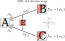
\includegraphics[draft=false, width=\linewidth]{qss/qss_distribution_stage}
		
	\end{subfigure}
	\begin{subfigure}{0.8\linewidth}
		\centering
		\caption{\label{fig:qss_encryption_stage}}
		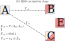
\includegraphics[draft=false, width=\linewidth]{qss/qss_encryption_stage}
		
	\end{subfigure}
\caption{\label{fig:qss_protocol_cartoon} Distribution and encryption stages of our QSS protocol. Alice (A) wishes to securely share her secret $\sigma_A$ amongst potentially dishonest recipients Bob (B) and Charlie (C). (a) Distribution stage. B and C send coherent states chosen from QPSK alphabet to Alice, who heterodynes and obtains outcomes $A_B, A_C$. Dishonest Eve will eavesdrop on the distribution of quantum states in order to gain information about $A_B, A_C$. (b) Encryption stage. Alice will form variable $X_A$ using her chosen function $\mathcal{F}$ with her heterodyne measurement outcomes as input variables. She converts $X_A$ to binary $\tilde{X}_A$ and encrypts the secret with it to reach $\varsigma_A = \sigma_A \oplus \tilde{X}_A$. The encrypted secret is then broadcast. Dishonest players are shown in red and honest players in gray. A combination of red and gray denotes uncertainty about dishonesty.
}
\end{figure}

Since Alice is the dealer who will decide on the eventual shared key our protocol is analogous to a reverse-reconciliation (RR) QKD system, and so we may similarly expect the performance benefits of RR QKD at high loss and noise. We note that having potentially untrusted players as the senders may open the protocol up to new classes of attack, for example if they are permitted to send a state which is outside the QPSK alphabet, and such attacks should be addressed in future work.

%\MT{talk somewhere about the types of attack we allow}


Our QSS protocol runs in three stages, a Distribution stage, an Encryption stage and, finally, a Decryption stage. Distribution and encryption stages are displayed in Fig.~\ref{fig:qss_protocol_cartoon}. The Distribution stage, Fig.~\ref{fig:qss_distribution_stage}, involves distribution and measurement of quantum coherent states chosen from QPSK alphabet. At the end of Distribution, Alice will hold classical information which is correlated with both Bob and Charlie. In the Encryption stage, Fig.~\ref{fig:qss_encryption_stage}, Alice will combine her classical information and use it to encode her sensitive classical secret. The encoded secret is distributed to Bob and Charlie. The secret is decoded by Bob and Charlie during Decryption. Our protocol setup is described in Fig.~\ref{fig:qss_structure},~\ref{fig:qss_protocol_cartoon}, and we describe it in detail below.

%\MT{make sure that the following is in the same style as my qds protocol description}

\subsubsection*{Distribution stage, Fig.~\ref{fig:qss_distribution_stage}}
\paragraph{Step $1$}
Alice wishes to encrypt a classical secret, $\sigma_A$. Bob forms a classical random variable $X_B = \left\{\phi_B\right\}$, where the $\phi_B$ are complex phases independently chosen from the QPSK alphabet. Phases $\phi_B$ are assumed to be chosen uniformly at random, but we relax this assumption in Chapter~\ref{chapter:aqc}. Charlie likewise forms classical random variable $X_C = \left\{\phi_C\right\}$.

\paragraph{Step $2$}
Bob and Charlie form sequences of coherent states based on their random variables
\begin{equation}
\rho\left[X_{\left(B, C\right)}\right] := \otimes \rho\left[\phi_{\left(B, C\right)}\right]
\end{equation}
where $\rho\left[\phi_{\left(B, C\right)}\right]$ denotes a coherent state with phase $\phi_{\left(B, C\right)}$. These sequences of states are sent to Alice through quantum channels. %\MT{Talk later about the types of channels which these are.}. 
Alice performs heterodyne detection, Sec.~\ref{sec:intro_heterodyne} on each of her received states and records her complex outcomes. We denote the strings of Alice's measurement outcomes as $A_B, A_C$, where $A_B$ corresponds to measurement outcomes from states sent by Bob, and $A_C$ corresponds to those on states sent by Charlie. The $A_B$ and $A_C$ are kept separate and secret, and Bob and Charlie should retain their information $X_B, X_C$.

\subsubsection*{Encryption stage, Fig.~\ref{fig:qss_encryption_stage}}

\paragraph{Step $3$} Alice creates a new string of complex variables
\begin{equation}
X_A = \mathcal{F}\left(A_B, A_C\right)
\end{equation}
from her measurement outcomes. The function $\mathcal{F}$ is chosen by Alice and should be freely chosen to optimize security. In this thesis we will pick simple forms for $\mathcal{F}$ which allow us to easily make concrete predictions about protocol security, although in general $\mathcal{F}$ may be as pathological as Alice desires.

% \MT{Where shall I talk about function $F$?} \MT{I can create some nice graphs of different functions $F$, even those requiring a lot of parameters to be optimized over. But when it comes to actually analysing security I should pick simple ones.} 

\paragraph{Step $4$} Alice now holds random variable $X_A$ of complex variables, which depends on both Bob and Charlie's choices $X_B, X_C$. Alice maps her string of complex variables onto a binary random variable $X_A \mapsto \tilde{X}_A$, and uses $\tilde{X}_A$ to encode $\sigma_A$ via an XOR operation. For ease we shall write this combined step in terms of an encryption function $\text{Enc}$, which should be known to all players at the start of the protocol. % I should probably talk about this later at some point?

\begin{equation}
\varsigma_A = \text{Enc}\left(\sigma_A, X_A\right)
\end{equation}

\noindent Alice distributes $\varsigma_A$ to Bob and Charlie, who are unable to access $\sigma_A$ since they do not yet know $X_A$.

\subsubsection*{Decryption stage}

\paragraph{Step $5$} Later, when Alice desires to allow Bob and Charlie access to $\sigma_A$, she broadcasts her choice of function $\mathcal{F}$, along with enough classical information to perform a reconciliation procedure between $X_A$ and $\mathcal{F}\left(X_B, X_C\right)$. This stage is similar to CV QKD and so we will not discuss it further. Bob and Charlie contribute their information $X_B, X_C$ to form $\mathcal{F}\left(X_B, X_C\right)$ and reconcile it to $X_A$ and thus $\tilde{X}_A$. Then they are able to access Alice's original secret $\sigma_A$.

Critical to the protocol is the fact that Alice forms a secret key based on a degree of freedom shared between Bob and Charlie, which forces collaboration. In this way, our protocol is a natural extension of the protocol from Kogias \emph{et. al.} \cite{Kogias2017}, and may be seen to help bridge the gap betwee entanglement-based and sequential QSS.

If either one of Bob or Charlie is dishonest, they are forced to work with an honest player and so our scheme has succeeded.



%\MT{some more remarks about the running of the protocol}


\section{Security against Eve}\label{sec:qss_honest_recipients}
%\MT{talk here about security against an external eavesdropper.}

The QSS protocol presented above must be secure against both the actions of an external eavesdropper and those of a dishonest Bob or Charlie who may be collaborating with Eve. We will first consider security against Eve in order to illustrate key steps from the security analysis, and so for this section we assume that Bob and Charlie are honest,
Fig.~\ref{fig:qss_honest_recipients}. In Sec.~\ref{sec:qss_dishonest_recipient} we will begin to allow for dishonesty in recipients Bob and Charlie.

\begin{figure}[htp]
\centering
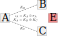
\includegraphics[draft=false, width=0.4\linewidth]{qss/qss_honest_recipients}
\caption{\label{fig:qss_honest_recipients} Alice will distribute her secret $\sigma_A$ to Bob and Charlie who are assumed honest. Dishonest Eve will try to attack the protocol and gain information about $\sigma_A$. Gray: honest. Red: dishonest. See Fig.~\ref{fig:qss_structure} for further information.}
\end{figure}


The starting point for our security analysis is the following Devetak-Winter bound \cite{Devetak2004} for the asymptotic key rate under collective attack, Fig.~\ref{fig:types_of_attack_collective},

%\MT{should I motivate why this bound is helpful for us?}

\begin{equation}\label{eqn:qss_dw_eve}
\kappa_{\text{Eve}} \ge \text{I}\left(X_A : X_B, X_C\right) - \chi\left(X_A : \mathbb{E}\right)
\end{equation}

\noindent which describes the balance between the mutual information, $\text{I}$, shared between Alice and a Bob-Charlie collaboration, and the Holevo information $\chi$ between Eve's quantum system $\mathbb{E}$ and Alice. It is perhaps unsurprising that Eq.~\ref{eqn:qss_dw_eve} should be our starting point given the noted similarities between QSS and QKD. The $X_A = \mathcal{F}\left(A_B, A_C\right)$ is Alice's variable based on her heterodyne measurement outcomes.

We would like to calculate the lower bound for key rate given by Eq.~\ref{eqn:qss_dw_eve} and so we will consider each term in turn and demonstrate how they may be calculated for the protocol described above.


\subsubsection{Mutual information}

Using Eq.~\ref{eqn:intro_mutual_information} the mutual information $\text{I}$ may be written as 
\begin{equation}\label{eqn:qss_deriv_1}
\text{I}\left(X_A : X_B, X_C\right) = \text{H}\left(X_B, X_C\right) - \text{H} \left(X_B, X_C \given X_A\right)
\end{equation}
where the first term on the right hand side is the joint Shannon entropy of $X_B$ and $X_C$, and the second term is the conditional Shannon entropy of $X_B, X_C$ given $X_A$. Intuitively this second term encodes the uncertainty one has about which $X_B, X_C$ were chosen, given a particular choice for $X_A$. 

The joint Shannon entropy may be written
\begin{equation}\label{eqn:qss_deriv_2}
\text{H}\left(X_B, X_C\right) = \sum_{X_B=b, X_C=c} - \text{P}\left(b, c\right) \log \text{P}\left(b, c\right)
\end{equation}
where $b, c$ are individual instances of variables $X_B, X_C$. The $b, c \in \mathcal{A}_4$. Since $b, c$ are taken to be independently chosen and uniformly random we see that the joint probability
\begin{equation}\label{eqn:qss_deriv_3}
\text{P}\left(b, c\right) = \text{P}\left(b\right)\times \text{P}\left(c\right) = \frac{1}{16}
\end{equation}
since each of the $b, c$ are chosen with probability $1/4$. 

Expanding the conditional probability in the prior \MT{is this the right term?} variable $X_A$ we reach

\begin{equation}\label{eqn:qss_deriv_4}
\text{H}\left(X_B, X_C \given X_A\right) = \int\limits_{a \in \mathbb{C}} \Diff2 a \; \text{P}\left(X_A = a\right) \text{H}\left(X_B, X_C \given X_A = a\right).
\end{equation}
Each term in Eq.~\ref{eqn:qss_deriv_4} can be calculated theoretically once function $F$ is known. 

We have no requirement that $F$ should be injective. In particular, this implies that \MT{X}. To be concrete, in what follows we assume that $F$ is linear
\begin{equation}\label{eqn:qss_F_linear}
F\left(x, y\right) := g x + h y \qq{with} g, h \in \mathbb{R}\setminus \left\{0\right\}
\end{equation} 
Although we make no claims about the optimality of this choice of $F$, we are free to optimize over $g, h$, and we will make it clear when we have done so. The conditional entropy in the integrand of Eq.~\ref{eqn:qss_deriv_4} expands as \MT{make equation look nice}

\begin{align}
\text{H}\left(X_B, X_C \given X_A\right) = \sum_{b, c \in \mathcal{A}_4} - &\text{P}\left(X_B=b, X_C=c \given X_A=a\right) \times \notag \\
%
&\log \text{P}\left(X_B=b, X_C=c \given X_A=a\right)
\end{align}

\noindent and so all that remains to calculate are the probabilities \begin{equation}
\text{P}\left(X_A=a\right) \qq{and} \text{P}\left(X_B=b, X_C=c \given X_A=a\right).
\end{equation}

\noindent Applying Bayes' formula to the second of these, we see that
\begin{equation}
\text{P}\left(X_B=b, X_C=c \given X_A=a\right) = \text{P}\left(X_A=a \given X_B=b, X_C=c\right) \frac{\text{P}\left(X_B=b, X_C=c\right)}{\text{P}\left(X_A=a\right)}.
\end{equation}
We can access $\text{P}\left(X_A=a \given X_B=b, X_C=c\right)$ by modelling the effects of the channel on quantum states distributed by Bob and Charlie, which we now do. We take
\begin{equation}\label{eqn:qss_deriv_5}
X_A = F\left(A_B, A_C\right) = g A_B + h A_C
\end{equation}
and thus
\begin{equation}
A_C = \frac{X_A - g A_B}{h}.
\end{equation}

\noindent Since our $F$ is not injective (there are multiple $A_B, A_C$ which will give the same $X_A$) we must average over all of the possible ways to reach a given $X_A$. Therefore, once $X_A$ is fixed, the choice of $A_B, A_C$ reduces to a one-variable problem and so

\begin{equation}
\text{P}\left(X_A \given X_B=b, X_C=c\right) = \int\limits_{A_B \in \mathbb{C}} \Diff2 A_B \; \text{P}\left(A_B , \frac{X_A - g A_B}{h} \given X_B=b, X_C=c\right)
\end{equation}
which may be calculated once we know how the channel acts on input states. A similar equation would be reached by rearranging Eq.~\ref{eqn:qss_deriv_5} as $A_B = \left(X_A - h A_C\right)/g$ but it will make no difference to the resulting quantities.

Assuming that the channel Charlie-Alice is independent from the channel Bob-Charlie\footnote{We shall see later what this physically corresponds to} allows us to write
\begin{equation}\label{eqn:qss_deriv_6}
\text{P}\left(A_B, A_C \given X_b=b, X_C=c\right) = \text{P}\left(A_B \given X_B=b\right) \times \text{P}\left(A_C \given X_C=c\right)
\end{equation}
for Alice's heterodyne measurement outcomes $A_B, A_C$. Let us assume for now that each channel is noiseless but lossy. The probability that Alice measures a particular heterodyne outcome $a \in \mathbb{C}$ when a coherent state of complex amplitude $\beta$ is sent through a lossy channel, transmittivity $T$, is 
\begin{equation}\label{eqn:qss_channel_classical_prob}
\frac{1}{\pi}\exp\left( - \left| a - \sqrt{T}\beta \right|^2\right)
\end{equation}
which we have used previously in Ch.~\MT{X}. The required changes to include thermal noise of the channel can be readily made.

The integral in Eq.~\ref{eqn:qss_deriv_6} may be calculated analytically to reach \MT{TODO: check this against my MMA file}
\begin{align}\label{eqn:qss_deriv_7}
\text{P}\left(X_A \given X_B=b, X_C=c\right) = \frac{1}{\pi} \frac{1}{g^2 + h^2} &\exp \left( - \frac{\left[b^R g \sqrt{T_B} + c^R h \sqrt{T_C} - X_A^R \right]^2}{g^2 + h^2}\right) \notag \\
%
&\exp \left( - \frac{\left[b^I g \sqrt{T_B} + c^I h \sqrt{T_C} - X_A^I \right]^2}{g^2 + h^2} \right)
\end{align}
where $b, c$ are Bob and Charlie's coherent state amplitudes, $X_A$ is Alice's final variable after applying $F$ to her heterodyne outcomes, $T_B, T_C$ are the transmittivities of the Bob-Alice channel and Charlie-Alice channel, respectively, and where a superscript $R\left(I\right)$ denotes the real (imaginary) part of the corresponding quantity. \MT{I probably don't need to say much about how this integration is actually done, since it should be obvious.} The probability $\text{P}\left(X_A=a\right)$ may be readily found by summing Eq.~\ref{eqn:qss_deriv_7} over $b, c \in \mathcal{A}_4$. 

Finally, the mutual information Eq.~\ref{eqn:qss_deriv_1} may be calculated. \MT{Q: do I explicitly perform the integral over $X_A$? If so then I should show it. Otherwise I should mention that it is performed numerically.}

Let us now explore how the mutual information behaves. \MT{Now let's make some graphs and really have fun exploring how $I$ behaves.}

\subsubsection{Holevo information}

We will now detail how the Holevo information term in Eq.~\ref{eqn:qss_dw_eve} may be calculated. In doing so we will point to areas where future work might strengthen the security analysis to wider classes of attack, which should help to illuminate the contexts to which our security proof may be applied. In this section we consider a dishonest Eve performing attack BS$0$, as detailed above in Sec.~\MT{X}, and more general attacks will be considered later.

Bob and Charlie prepare a state from QPSK alphabet with equal probability. The coherent states should be independently and randomly chosen. Before the channel they hold the joint state
\begin{equation}
\rho_{\text{before}} = \rho_B \otimes \rho_C
\end{equation}
with
\begin{equation}
\rho_B = \frac{1}{4} \sum_{k=0}^3 \dyad{\beta_k}_B \qq{and} \rho_C = \frac{1}{4} \sum_{k^\prime = 0}^3 \dyad{\gamma_{k^\prime}}_C
\end{equation}
where $\beta, \gamma$ are the amplitudes of Bob's and Charlie's coherent state alphabets.\footnote{Complex amplitudes $\beta, \gamma$ were denoted $b, c$ in the previous section.}

We assume that the channel acts separately on each mode, and that modes $\rho_B$, $\rho_C$ undergo independent evolution. In other words, we assume that the channel has tensor-product structure
\begin{equation}
\Phi\left[\rho\right] = \Phi_B\left[\rho\right] \otimes \Phi_C\left[\rho\right]
\end{equation}
where \MT{check this equation}
\begin{equation}
\Phi_B\left[\rho\right] = \phi_B\left(\text{Tr}_B \rho\right) \otimes \mathbb{1}\left(\rho\right).
\end{equation}

\noindent Eve performs separate beamsplitter attacks on each channed and retains two output modes $\mathbb{E}_{B, C}$. The total state after the channel becomes
\begin{equation}
\rho_{\text{after}} = \rho_{\mathbb{A}_B, \mathbb{E}_B} \otimes \rho_{\mathbb{A}_C, \mathbb{E}_C}
\end{equation}
with $\mathbb{A}_{B, C}$ denoting Alice's two modes and where
\begin{equation}
\rho_{\mathbb{A}_B, \mathbb{E}_B} = \frac{1}{4} \sum_{k=0}^3 \dyad{\sqrt{T_B} \beta_k}_{\mathbb{A}_B} \otimes \dyad{\sqrt{1-T_B} \beta_k}_{\mathbb{E}_B}
\end{equation}
and similarly for $\rho_{\mathbb{A}_C, \mathbb{E}_C}$. Now, Alice heterodynes and measures $A_B \in \mathbb{C}$ from $\rho_{\mathbb{A}_B, \mathbb{E}_B}$ and $A_C \in \mathbb{C}$ from $\rho_{\mathbb{A}_C, \mathbb{E}_C}$. Eve's total state conditioned on these outcomes becomes 
\begin{equation}
\rho_{\left.\mathbb{E} \given A\right.} = \rho_{\left.\mathbb{E}_B \given A_B\right.} \otimes \rho_{\left. \mathbb{E}_C \given A_C\right.}
\end{equation}
with
\begin{equation}
\rho_{\left.\mathbb{E}_B \given A_B\right.} = \frac{1}{4 \pi} \sum_{k=0}^3 \text{P}_B\left(A_B \given \beta_k, T_B\right) \dyad{\sqrt{1-T_B} \beta_k}_{\mathbb{E}_B}
\end{equation}
and similarly for $\rho_{\left.\mathbb{E}_C \given A_C\right.}$. The probability $\text{P}_B\left(A_B \given \beta_k, T_B\right)$ is calculated analogously to Eq.~\ref{eqn:qss_channel_classical_prob}, and similarly for $A_C$.

Take $X_A = g A_B + h A_C$ as usual, with $g, h$ fixed, and write $A_C = \left(X_A - g A_B\right)/h$. Therefore we have

\begin{align}\label{eqn:qss_deriv_8}
\rho_{\left. \mathbb{E} \given X_A, A_B\right.} &= \frac{1}{16 \pi^2} \sum_{k, k^\prime = 0}^3 \text{P}_B\left(A_B \given \beta_k, T_B\right) \text{P}_C\left(\frac{X_A - g A_B}{h} \given \gamma_{k^\prime}, T_C\right) \notag \\
%
&\dyad{\sqrt{1-T_B} \beta_k}_{\mathbb{E}_B} \otimes \dyad{\sqrt{1-T_C}\gamma_{k^\prime}}_{\mathbb{E}_C}
\end{align}

\noindent Once again since Alice's function $F$ is in general not injective, we must mix over outcomes $A_B, A_C$ in order to find Eve's state $\rho_{\left.\mathbb{E} \given X_A\right.}$

\begin{equation}\label{eqn:qss_aposteriori_state}
\rho_{\left.\mathbb{E} \given X_A\right.} = \int\limits_{A_B \in \mathbb{C}} \Diff2 A_B \; \text{P}\left(A_B\right) \rho_{\left.\mathbb{E} \given X_A, A_B\right.}
\end{equation}

\noindent and mixing over $X_A$ we finally reach

\begin{equation}\label{eqn:qss_apriori_state}
\rho_{\mathbb{E}} = \int\limits_{X_A \in \mathbb{C}} \Diff2 X_A \; \text{P}\left(X_A\right) \rho_{\left.\mathbb{E}\given X_A\right.}.
\end{equation}

\noindent We may identity Eq.~\ref{eqn:qss_aposteriori_state} as Eve's \emph{a prosteriori} state and Eq.~\ref{eqn:qss_apriori_state} as Eve's \emph{a priori} state and so Eve's Holevo information is given by the usual formula

\begin{equation}\label{eqn:qss_holevo}
\chi = \text{S}\left(\rho_\mathbb{E}\right) - \int\limits_{X_A \in \mathbb{C}} \Diff2 X_A \; \text{P}\left(X_A\right) \text{S}\left(\rho_{\left.\mathbb{E} \given X_A\right.}\right).
\end{equation}

\noindent Let us explore the behaviour of Eve's Holevo information Eq.~\ref{eqn:qss_holevo}.

\MT{TODO: make some nice graphs of $\chi$ in different scenarios and under different attacks BS1, BS2, EC.}

\section{Security against a dishonest player}
\MT{Talk about guarding against a dishonest Bob/Charlie.}
Including a dishonest player, Bob or Charlie, in the above security proof requires us to re-calculate several quantities from the above section. For concreteness we will first assume that Bob is dishonest and Charlie is honest, and we allow Bob to collaborate with Eve. Later we will discuss how to account for the fact that we do not know \emph{which} player is dishonest.

The effect of including a dishonest player is that Bob knows precisely which coherent states he sent to Alice, and so he should have reduced uncertainty (increased Holevo information) about $X_A$. Intuitively it is also possible that Bob could wait and see which coherent states Charlie sent before choosing his own, in order to preference a certain outcome $X_A$. \MT{Make a comment about this. Would it be taken care of by Alice's optimization over $g, h$?} We will also assume that Bob sends states from his QPSK alphabet, though this could be relaxed in future work.

Since Bob knows which coherent states he sent we must re-calculate several expressions from the previous section. \MT{talk about which ones should be changed.} The key change throughout is that we should no longer mix over Bob's alphabet. This is easily taken into account in the calculation of mutual information, and since the calculation above was left quite general we will not reproduce the steps here.

Holevo information is calculated likewise, with Eve's state conditioned on $X_A, A_B$ given by
\begin{align}\label{eqn:qss_deriv_9}
\rho_{\left.\mathbb{E} \given X_A, A_B\right.} = \frac{1}{4 \pi^2} \sum_{k^\prime=0}^3 \text{P}_B\left(A_B \given \beta_k, T_B\right) \text{P}_C\left(\frac{X_A - g A_B}{h} \given \gamma_{k^\prime}, T_C\right) \notag \\
%
&\dyad{\sqrt{1-T_B} \beta_k}_{\mathbb{E}_B} \otimes \dyad{\sqrt{1-T_C}\gamma_{k^\prime}}_{\mathbb{E}_C}
\end{align}
(c.f. Eq.~\ref{eqn:qss_deriv_8}) and the \emph{a posteriori} and \emph{a priori} states calculated by integrating Eq.~\ref{eqn:qss_deriv_9} identically to Eqs.~\ref{eqn:qss_aposteriori_state},~\ref{eqn:qss_apriori_state}.

\MT{Chat about the fact that we don't actually know which player is dishonest.}

\MT{Make some graphs looking at mutual information and Holevo information}


\section{Protocol performance}
\MT{Make some graphs of key rate and tweak all of the parameters that I can in all of the attacks that I can.}

\MT{If I have time, make some graphs with e.g. homodyning instead of heterodyning, or different alphabets.}

























\section{Outlook}
\MT{this section should be somewhere else, perhaps in an "outlook" section?}
The classical post-processing of the above protocol is inherently very similar to Ref.~\cite{Kogias2017}, in which a secret key is generated between Alice and a shared Bob-Charlie degree of freedom via incompatible homodyne measurements on a tripartite entangled state. We expect that our protocol will be secure against a more restricted set of attacks, but over a wider range of channel parameters, for several reasons. 

Ref.~\cite{Kogias2017} has potentially dishonest players Bob and Charlie performing homodyne measurements on incompatible observables (i.e. switching between $q$ and $p$ quadratures). No assumptions are made about the measurement devices used and they are each treated as a "black-box". Security comes inherently because of a Heisenberg-type relation between incompatible observables, and the security proof relies on an Entropic Uncertainty Relation (EUR). These EURs have had success elsewhere in quantum cryptography \MT{cite}. However, since we desire to use heterodyne detection we are forced to adopt a different approach and explicitly model the states' evolution and measurement during the protocol. We note that this matches the current state-of-the-art of QPSK-based QKD, but can be improved in future work.

We have assumed that a dishonest Bob or Charlie still sends a state from the QPSK alphabet. It is yet unclear whether they could gain an advantage by sending something exotic and potentially highly entangled, perhaps in order to force Alice to reach a certain key $X_A$. This should be explored and potentially relaxed in future work. We anticipate that applying methods from quantum bit commitment might prove fruitful here. 

Finally, we note that our assumption that the channel between Alice and Bob-Charlie takes a tensor-product structure is perhaps a strong one and should be relaxed. A potential strategy of a dishonest player could be to exploit properties of a general channel which maps a two-mode input state to a two-mode output state at Alice, though potentially allowing a dishonest player many output ancilla modes correlated with Alice. Such a strategy will be restricted by the conditions that the reduced state of an honest player should be a coherent state. Similarly it will require that Alice's measurement outcomes don't look errant, though this should be quantified.








